\documentclass[twoside]{report}

% Sets up the document template, imports needed packages and other useful ones, and defines some useful commands

\usepackage[printonlyused]{acronym}
\usepackage{amsmath}
\usepackage{breqn}
\usepackage[blocks]{authblk}
\usepackage[backend=biber,sorting=none]{biblatex}
\usepackage[justification=justified,singlelinecheck=off,bf]{caption}
\usepackage{chngcntr}
\usepackage{changepage}
\usepackage[usenames,dvipsnames]{color}
\usepackage{enumerate}
\usepackage{enumitem}
\usepackage{fancyhdr}
\usepackage{fancybox}
\usepackage{fancyvrb}
\usepackage{float}
\usepackage{framed}
\usepackage{placeins}
\usepackage[top=1.5in,bottom=1.5in,inner=1.0in,outer=1.0in,headheight=50pt,footskip=50pt,headsep=40pt]{geometry}
\usepackage{graphicx}
\usepackage{lastpage}
\usepackage{lscape}
\usepackage{multirow}
\usepackage{units}
\usepackage{newfloat}
\usepackage{wrapfig}
\usepackage{multicol}
\usepackage{tablefootnote}
\usepackage{hyperref}
\usepackage{tabularx}
\usepackage{siunitx}
\usepackage{textcomp}
\usepackage[pages=some]{background}
\usepackage{longtable}
\usepackage{booktabs}
\usepackage{titlesec}
\usepackage{listings}
\usepackage[titletoc,title]{appendix}
\usepackage{colortbl}
\usepackage{nomencl}
\usepackage{sectsty}


%customize hyperref
%uncomment to underline the hyperlinks in the document
\hypersetup{
        colorlinks,
%	colorlinks=false,
%	pdfborderstyle={/S/U/W 1},
%	pdfborder=0 0 1,
	linkcolor=black,
	citecolor=black,
	}


% Make custom blue to match word blue
\definecolor{DocNameBlue}{RGB}{154,189,251}
% CASL blue
\definecolor{CASLBlue}{RGB}{0,132,246}
\definecolor{TitleBlue}{RGB}{37,65,96}
\definecolor{codegreen}{rgb}{0,0.6,0}
\definecolor{codegray}{rgb}{0.5,0.5,0.5}
\definecolor{codepurple}{rgb}{0.58,0,0.82}
\definecolor{backcolour}{rgb}{0.9,0.9,0.9}
\definecolor{caslcolor1}{HTML}{E9EDF4}
\definecolor{caslcolor2}{HTML}{D0D8E8}
\definecolor{caslheader}{HTML}{4F81BD}


% All the other pages style
\renewcommand{\headrulewidth}{0pt}
\fancyhead{}
\fancyfoot{}
\fancyhead[LO,RE]{
\includegraphics[width=1.5in]{template/CASL_logo.png}}
\fancyhead[RO,LE]{\color{CASLBlue}\shortTitle}
\fancyfoot[LE,RO]{\textcolor{CASLBlue}{C}onsortium for \textcolor{CASLBlue}{A}dvanced \textcolor{CASLBlue}{S}imulation of \textcolor{CASLBlue}{L}WRs}
\fancyfoot[RE,LO]{\CASLMilestoneNumber}
\fancyfoot[CO,CE]{\thepage}

\fancypagestyle{plain}
{
\fancyhead[LO,RE]{
\includegraphics[width=1.5in]{template/CASL_logo.png}}
\fancyhead[RO,LE]{\color{CASLBlue}\shortTitle}
\fancyfoot[LE,RO]{\textcolor{CASLBlue}{C}onsortium for \textcolor{CASLBlue}{A}dvanced \textcolor{CASLBlue}{S}imulation of \textcolor{CASLBlue}{L}WRs}
\fancyfoot[RE,LO]{\CASLMilestoneNumber}
\fancyfoot[CO,CE]{\thepage}
}

% The title page style
\fancypagestyle{firststyle}
{
   \fancyhead[L]{}
   \fancyhead[R]{\CASLMilestoneNumber}
   \fancyfoot[]{}
}



\backgroundsetup{
scale=1,
color=black,
opacity=1.0,
angle=0,
contents={%
  
\includegraphics[width=\paperwidth,height=\paperheight]{template/casl_background.pdf}
  }%
}

% Define command to surround text in angle brackets
\newcommand{\brackets}[1]{\textlangle{}#1\textrangle{}}

% For formatting code
\newcommand{\codeblock}[1]{\texttt{#1}}

%increase space after captions
\setlength{\belowcaptionskip}{2pt}

% No indenting at start of paragraph
\setlength{\parindent}{0pt}

%increase space between paragraphs
\parskip 1em

\titleformat{\chapter}{\Huge\bfseries}{\thechapter. }{0pt}{\Huge\bfseries}

% set the section numbering depth and TOC depth
\setcounter{secnumdepth}{3}
\setcounter{tocdepth}{3}

% Use continuous counting scheme for floats
\counterwithout{table}{chapter}

\let\DeclareUSUnit\DeclareSIUnit
\let\US\SI
\DeclareUSUnit\F{F}
\DeclareUSUnit\ft{ft}
\DeclareSIUnit\inch{in}

%define the degree command for using temperature units
\providecommand{\degree}{\ensuremath{^{\circ}}}

% define new command to make custom vector notation
\newcommand{\vect}[1]{\vec{#1}}

% define a command to correct subscript size
\newcommand{\smallsub}[1]{\scriptscriptstyle{\text{#1}}}

% Define a macro to make the "by" symbol 
\newcommand{\by}{\texorpdfstring{\ensuremath{\times}}{x}}

% define command for quick scientific notation
\providecommand{\e}[1]{\ensuremath{\cdot10^{#1}}}

\newcommand{\CASLMilestoneNumber}{CASL-2019-1884-001}
\title{VERAIn Programmer Manual}
\newcommand{\shortTitle}{VERAIn Programmer Manual}
\newcommand{\subtitle}{}
\newcommand{\psm}{Erik Walker, VERAIO Product Software Manager}
\newcommand{\reviewer}{Independent Reviewer}
\newcommand{\publicationDate}{11/11/2019}


\author[1]{E. Walker}

\affil[1]{Oak Ridge National Laboratory}


\begin{document}

%clear the header/footer until TOC
\pagenumbering{roman}

\begin{titlepage}

\begin{titlepage}

   \BgThispage
   \thispagestyle{firststyle}
   
   \vspace*{\fill}
   
   \begin{minipage}[l][][c]{0.6\textwidth}
   \begin{flushleft}
   \makeatletter
   {\huge\color{TitleBlue}\bf Consortium for Advanced \\\vspace{0.3cm} Simulation of LWRs}\\
   \vspace{3cm}
   {\huge\fontfamily{phv}\selectfont\color{TitleBlue}\bf
   % Title of the document
   \@title\par
   }
   {\Large\fontfamily{phv}\selectfont\color{DocNameBlue}\bf
   \subtitle\par
   }
   \vspace*{30pt}
   % Authors
   {\Large\bf\setlength{\parskip}{10pt}
   \@author
   
   }
   \vspace*{30pt}
   {\huge\bf
   \publicationDate
   }
   \makeatother
   
   
   \end{flushleft}
   \end{minipage}
   
   \vspace*{\fill}
   
\begin{minipage}{0.6\textwidth}
   
\includegraphics[width=\textwidth]{template/verabanner.png}
\end{minipage}

   
   \end{titlepage}

   \pagestyle{fancy}

   \vspace*{\fill}

   \captionsetup{justification=centering}
   \begin{table}[H]
   \centering
   \caption*{\Large\bfseries{Revision Log}}
   \begin{tabular}{rrrr}
   \toprule
   \textbf{Revision} & \textbf{Date} & \textbf{Affected Pages} & \textbf{Revision Description} \\
   \midrule
   0 & \publicationDate & All & Initial Release \\
   & & & \\
   & & & \\
   & & & \\
   & & & \\
   & & & \\
   & & & \\
   \bottomrule
   \end{tabular}
   \end{table}
   
   \vspace*{\fill}
   
   
   \begin{table}[H]
   \caption*{\Large\bfseries{Document pages that are:}}
   \centering
   \begin{tabular}{ll}
   Export Controlled: & None \\
   IP/Proprietary/NDA Controlled: & None \\
   Sensitive Controlled: & None \\
   Unlimited: & All \\
   \end{tabular}
   \end{table}
   
   \vspace*{\fill}
   
   This document was prepared as an account of work sponsored by an agency of the United States Government. Neither the United States Government nor any agency thereof, nor any of their employees, makes any warranty, express or implied, or assumes any legal liability or responsibility for the accuracy, completeness, or usefulness of any information, apparatus, product, or process disclosed, or represents that its use would not infringe privately owned rights. Reference herein to any specific commercial product, process, or service by trade name, trademark, manufacturer, or otherwise, does not necessarily constitute or imply its endorsement, recommendation, or favoring by the United States Government or any agency thereof. The views and opinions of authors expressed herein do not necessarily state or reflect those of the United States Government or any agency thereof.

   \captionsetup{justification=justified}
   
   \vspace*{\fill}
   
   \newpage

\end{titlepage}

\clearpage 

\makeatletter
\begin{center}
{\huge\bf\@title\par}
\end{center}

\vspace{2cm}

{\Large\bf Approvals:}

\vspace{2cm}

\begin{tabular}{ll}
\makebox[3.5in]{\hrulefill} & \makebox[2.0in]{\hrulefill}\\
{\bf\psm} & {\bf Date}\\[3cm]

\makebox[3.5in]{\hrulefill} & \makebox[2.0in]{\hrulefill}\\
{\bf\reviewer} & {\bf Date}\\[3cm]

\end{tabular}

\makeatother

\clearpage

\addcontentsline{toc}{section}{Executive Summary}
\chapter*{Executive Summary}

This document provides information needed by developers who will be working in the VERAIn source code. 
It provides a high-level overview of input design as well as guidelines for adding new inputs.

\tableofcontents

\listoffigures

\clearpage
\pagenumbering{arabic}
\pagestyle{fancy}

\acresetall

\pagenumbering{arabic}



\chapter{VERAIn}

The VERAIn repository is used to translate the user defined ASCII input file to a ParameterList XML file to be read by VERA. 
The ParameterList format is defined in Trilinos Teuchos package at:\\
\texttt{https://trilinos.org/docs/dev/packages/teuchos/doc/html/index.html\#TeuchosParameterList_src}.
The VERAIn parser is a PERL script that translates individual variables that are specified in YAML files. 
These YAML files are located in the \texttt{VERAIO/verain/scripts/Templates} directory.
To perform the translation, use the parser located in the scripts directory. 
Run the parser with a command line like the following:

\texttt{VERAIO/verain/scripts/react2xml.pl \$CASE.inp \$CASE.xml}

where \texttt{\$CASE} is the base name of your input file. 
Parser error messages indicate errors in the input file. 
More verbose diagnostic messages are currently being added. 
Various input parameter examples can be found in the \texttt{VERAIO/verain/test} directory.


\chapter{Style Guide}

\section{Adding New Variables}

This section provides instructions for adding or modifying inputs to be used in the user provided ASCII input. For most cases, to add a new variable to the input, only the template files found in \texttt{VERAIO/verain/scripts/Templates} need to be modified. Generally, two files need to be modified for every new input variable:
\begin{itemize}
    \item{Directory.yml} --- gives a description of how to read the input cards
    \item{BLOCK.yml} --- gives a description of how to convert input cards to parameter names for a particular BLOCK
\end{itemize}

The different BLOCK options that are available in an input file are:

\texttt{STATE, CORE, ASSEMBLY, CONTROL, INSERT, DETECTOR, EDITS, SHIFT, COBRATF, COUPLING, MPACT, BISON, MAMBA, and RUN}

For example, if a new variable is to be added to the ASSEMBLY block of the user input, it would need to be added to the ASSEMBLY section of the Directory.yml file as well as to the ASSEMBLY.yml file. 

Whenever a new variable is added to the Directory.yml file, proper documentation must also be provided. The input description must precede the variable and be of the following form using \LaTeX\ formatting:

\begin{verbatim}
#>
#>   {\bf variable\_name} detailed\_input\_name
#>   \VERAInputTable{
#>     name={detailed\_input\_name},
#>     type={variable type: Float, Boolean, Integer... etc.},
#>     need={Optional or Required},
#>     unitsdefault={Default units for this variable},
#>     unitsother={Other acceptable units for this variable},
#>     valuedefault={Default value for this variable, if there is one},
#>     valuesapplicable={Defines acceptable values, or range of values, that this variable 
#>        can be defined as},
#>     limitations={A description of the limitations of this variable, if applicable},
#>     description={A detailed description of this variable and what it is used for.},
#>     notes={Any additional information about this variable that was not specified earlier}
#>   }
\end{verbatim}

It is strongly advised that a new variable include a \texttt{_check:} section that checks to make sure that a given variable is the proper type and within the expected input variable range. An example of a two-variable input card with description is shown in Figure \ref{fig:Directory_example}. This example input, \texttt{b10}, is located in STATE block. Therefore, the corresponding entries in the STATES.yml file are shown in Figure \ref{fig:States_example}. The names given in the BLOCK.yml file will correspond to the variable name that will given in the ParameterList XML file. 

\begin{figure}
   \centering
   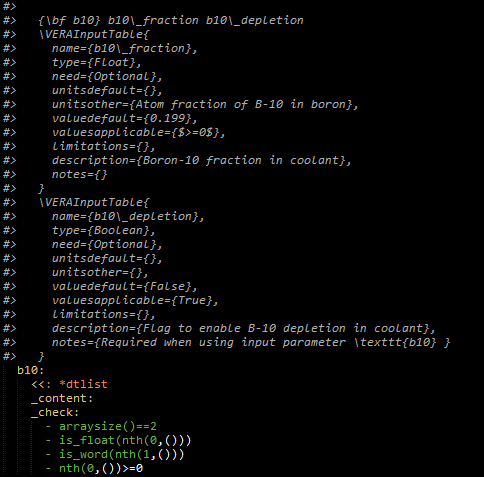
\includegraphics[width=\textwidth]{images/Directory_example}
   \caption{\label{fig:Directory_example}Example b10 inputs and descriptions in Directory.yml}
\end{figure}

\begin{figure}
   \centering
   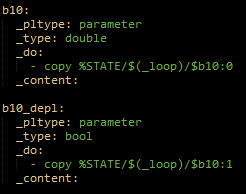
\includegraphics[width=10cm]{images/States_example}
   \caption{\label{fig:States_example}Example b10 inputs in STATES.yml }
\end{figure}
   
\section{Testing New Variables}

Whenever a new input card is added, a test case must also be added.
To add a test case, either modify an existing test case or add a new one in the \texttt{VERAIO/verain/test} directory.
It is preferable to modify an existing case, but care must be taken not to impact another test that might use the same case.

There is a special test input deck called \texttt{misc\_options.inp} that contains a bunch of random input variables. 
The only purpose of this test is to make sure something gets written to the XML file correctly.
If possible, try to use this test case instead of creating something new.
Once a test case has been either modified or created, a "gold" xml file must be created to go along with it.
If a new test is added, be sure to modify the \texttt{CMakeLists.txt} file in the \texttt{VERAIO/verain/test} directory and add another entry to the long list of \texttt{ADD\_REACTOR\_AWARE\_INPUT\_PARSER\_TEST} cases.

\chapter{VERARun}

VERARun is a set of Python scripts that allow for the easy execution of problems in VERA. 
The scripts are located in the VERAIO repository in the \texttt{VERAIO/verarun} directory.

To execute a problem using VERARun, a user simply types:
\begin{Verbatim}
    verarun $CASE
\end{Verbatim}

Additional command line options can be found by typing {\tt verarun} with no arguments.
Doing so will return the following options.

\begin{Verbatim}[fontsize=\small]
usage: verarun [-x] [-e email_addr] [-h] [-c config_file] [-N job_name] [-l]
               [-n nprocs] [-O] [--ppn cpus_per_node] [-m mem_per_process]
               [-s subdir] [-d vera_install_dir] [-v vera_version] [--verbose]
               [-W] [-w job_id] [-t walltime] [--chain] [--debug]
               [--hostname host] [-r {overwrite,readwrite}]
               [--vera-installs-dir vera_installs_dir]
               [input_path [input_path ...]]

Creates and optionally submits machine-specific VERA jobs.

positional arguments:
  input_path            path to VERA input (.inp) or XML (.xml) files

optional arguments:
  -x, --dry-run         dry run only, create but don't execute the PBS script
  -e email_addr, --email-addrs email_addr
                        comma-delimited list of email addresses to notify of
                        job completion, defaults to ${USER}@$(hostname)
  -h, --help            print detailed help
  -c config_file, --host-config-file config_file
                        override host configuration file, supercedes
                        --hostname and --vera-installs-dir
  -N job_name, --job-name job_name
                        name for the PBS job
  -l, --list-vera-versions
                        list available VERA versions
  -n nprocs, --np nprocs, --nprocs nprocs, --num-procs nprocs
                        total number of processors need for the job (mpiexec
                        -np param), defaults to value computed from input
  -O, --output-job-name
                        print the job name to stdout
  --ppn cpus_per_node, --pnode cpus_per_node
                        specify processors per node, by default this is
                        calculated
  -m mem_per_process, --pmem mem_per_process, --proc-memory mem_per_process
                        specify memory required per processor in GB, defaults
                        to undefined
  -s subdir, --subdir subdir
                        create subdir, a value of "." specifies automatically
                        generated subdir name
  -d vera_install_dir, --vera-dir vera_install_dir
                        path to VERA installation, superceding --vera-
                        installs-dir, --vera-version, and the host
                        configuration
  -v vera_version, --vera-version vera_version
                        name of VERA version to use
  --verbose             turn on verbose messaging
  -W                    wait on job last submitted via verarun, overrides -W
  -w job_id, --wait-job-id job_id
                        ID of job which must complete before starting this job
  -t walltime, --wall-time walltime
                        wallclock execution time in floating point hours,
                        defaults to 24.0

advanced arguments:
  --chain, --chain-jobs
                        each case depends on its predecessor
  --debug               debug mode
  --hostname host       force the hostname
  -r {overwrite,readwrite}, --restart {overwrite,readwrite}
                        optional restart mode
  --vera-installs-dir vera_installs_dir
                        path to vera_installs directory containing VERA
                        versions

\end{Verbatim}

%%%%%%%%%%%%%%%%%%%%%%%%%%%%%%%%
\section{VERARun Output}

Upon completion of a VERA job, several output files may be created depending on the code options used.
Some typical outputs include:
\begin{itemize}
\item VERAIn XML file.  This file is written upon the successful completion of VERAIn
\item VERA HDF output file.  This is a binary file with results that can be visualized in VERAView, or post-processed with user utility codes.
\item MPACT output file.  This file is written upon the successful completion of MPACT (if applicable).
\item MPACT log File.  This file is written upon the successful completion of MPACT (if applicable).
\item MPACT summary File.  This file is written upon the successful completion of MPACT (if applicable).
\item Standard output file. This file is a log of all output written to the standard output.
\item Standard error file.  this file is a log of all output written to the standard error file.
\end{itemize}


In case of errors, the user should examine the standard error file first.
If there were any errors in the input processor (VERAIn), the errors will be written here.
Any error messages from other VERA components will also be written to the standard error file.

If the standard error file does not list any errors, example the VERA component output files and log files for messages.


\end{document}
